
\section{Dati d'esempio}

	Esistono 6 file di dati d'esempio che prendono le immagini da 3 set distinti; a coppie, i file richiedono la soluzione su uno stesso set di immagini, ma con parametri diversi. \\
	Per ogni set vengono presentati i dati distinti con i parametri utilizzati nei relativi file. Quindi si mostrerà l'output del programma \texttt{amplide} seguito dai valori delle variabili della soluzione. \\
	La soluzione si compone del valore della funzione obiettivo, che coincide con la variabile D, seguito da una tupla nel formato <nome, X, Y, larghezza, altezza, rotazione> per ogni immagine. \\
	Seguirà poi un confronto grafico tra le soluzioni dei vari problemi con parametri diversi.


%%%%%%%%%%
%% SET 1
%%%%%%%%%%

	\subsection{Set 1}
Dati del set di immagini:  \\

\begin{table}[H]
\centering
\footnotesize
\begin{tabular}{l|r|r}
\multicolumn{3}{c}{\textbf{Immagini}} \\ 
%\hline
id & larghezza & altezza \\
\hline
a & 16 & 16 \\
b & 8&16\\
c & 8& 8\\
d & 5&25\\
e & 72&32\\
f & 32 &32\\
\end{tabular}
\end{table}


\noindent Parametri, Output e Soluzione dei 2 problemi: 

\begin{table}[H]
\centering
\footnotesize
\begin{tabular}{p{6cm}|p{6cm}}
%\hline
\textbf{Problema 1} & \textbf{Problema 2} \\ 
\hline
\multicolumn{2}{|c|}{Parametri} \\ 
\hline
allowRotations = 0,\newline
useNoBleeding = 0,\newline
usePowersOf2 = 1;	& 
allowRotations = 1,\newline
useNoBleeding = 1,\newline
usePowersOf2 = 1;	\\
\hline
\multicolumn{2}{|c|}{Output AMPL} \\
\hline
\texttt{114 MIP simplex iterations\newline
0 branch-and-bound nodes\newline
D = 128}
&
\texttt{110 MIP simplex iterations\newline
0 branch-and-bound nodes\newline
D = 128}
\\
\hline
\multicolumn{2}{|c|}{Soluzione} \\
\hline
\texttt{128\newline
'a',93,0,16,16,0\newline
'b',85,0,8,16,0\newline
'c',77,0,8,8,0\newline
'd',72,0,5,25,0\newline
'e',0,0,72,32,0\newline
'f',0,32,32,32,0}
&
\texttt{128\newline
'a',0,27,18,18,0\newline
'b',0,17,18,10,1\newline
'c',0,7,10,10,0\newline
'd',0,0,27,7,1\newline
'e',28,0,74,34,0\newline
'f',0,45,34,34,0}
\\
   
\end{tabular}
\end{table}

























%%%%%%%%%%
%% SET 2
%%%%%%%%%%

	\subsection{Set 2}
Dati del set di immagini:  \\

\begin{table}[H]
\centering
\footnotesize
\begin{tabular}{l|r|r}
\multicolumn{3}{c}{\textbf{Immagini}} \\ 
%\hline
id & larghezza & altezza \\
\hline
a & 128 & 32 \\
b & 32&32\\
c & 64& 64\\
d & 96&32\\
e & 32&64\\
f & 168 &32\\
g & 96&128\\
h & 96& 96\\
\end{tabular}
\end{table}


\noindent Parametri, Output e Soluzione dei 2 problemi: 

\begin{table}[H]
\centering
\footnotesize
\begin{tabular}{p{6cm}|p{6cm}}
%\hline
\textbf{Problema 3} & \textbf{Problema 4} \\
\hline
\multicolumn{2}{|c|}{Parametri} \\ 
\hline
allowRotations = 1,\newline
useNoBleeding = 1,\newline
usePowersOf2 = 0;	& 
allowRotations = 0,\newline
useNoBleeding = 0,\newline
usePowersOf2 = 0;	\\
\hline
\multicolumn{2}{|c|}{Output AMPL} \\
\hline
\texttt{16295 MIP simplex iterations\newline
2405 branch-and-bound nodes\newline
D = 228}
&
\texttt{1084 MIP simplex iterations\newline
277 branch-and-bound nodes\newline
D = 224}
\\
\hline
\multicolumn{2}{|c|}{Soluzione} \\
\hline
\texttt{228\newline
'a',98,0,130,34,0\newline
'b',194,100,34,34,0\newline
'c',132,34,66,66,0\newline
'd',132,100,34,98,1\newline
'e',194,134,34,66,0\newline
'f',98,58,34,170,1\newline
'g',0,98,98,130,0\newline
'h',0,0,98,98,0}
&
\texttt{224\newline
'a',32,0,128,32,0\newline
'b',192,0,32,32,0\newline
'c',96,64,64,64,0\newline
'd',0,192,96,32,0\newline
'e',0,0,32,64,0\newline
'f',56,32,168,32,0\newline
'g',0,64,96,128,0\newline
'h',97,128,96,96,0}
\\
\end{tabular}
\end{table}













\newpage


%%%%%%%%%%
%% SET 3
%%%%%%%%%%

\subsection{Set 3}
Dati del set di immagini:  \\

\begin{table}[H]
\centering
\footnotesize
\begin{tabular}{l|r|r}
\multicolumn{3}{c}{\textbf{Immagini}} \\ 
%\hline
id & larghezza & altezza \\
\hline
a & 16 & 32 \\
b & 32&32\\
c & 8& 8\\
d & 5&15\\
e & 32&64\\
f & 168 &32\\
g & 96&128\\
h & 96& 96\\
\end{tabular}
\end{table}


\noindent Parametri, Output e Soluzione dei 2 problemi: 

\begin{table}[H]
\centering
\footnotesize
\begin{tabular}{p{6cm}|p{6cm}}
%\hline
\textbf{Problema 5} & \textbf{Problema 6} \\
\hline
\multicolumn{2}{|c|}{Parametri} \\ 
\hline
allowRotations = 1,\newline
useNoBleeding = 1,\newline
usePowersOf2 = 0;	& 
allowRotations = 1,\newline
useNoBleeding = 1,\newline
usePowersOf2 = 1;	\\
\hline
\multicolumn{2}{|c|}{Output AMPL} \\
\hline
\texttt{4403 MIP simplex iterations\newline
1423 branch-and-bound nodes\newline
D = 198}
&
\texttt{222 MIP simplex iterations\newline
0 branch-and-bound nodes\newline
D = 256}
\\
\hline
\multicolumn{2}{|c|}{Soluzione} \\
\hline
\texttt{198\newline
'a',180,0,18,34,0\newline
'b',164,164,34,34,0\newline
'c',170,0,10,10,0\newline
'd',169,83,7,17,0\newline
'e',136,0,34,66,0\newline
'f',0,0,34,170,1\newline
'g',34,100,130,98,1\newline
'h',34,0,98,98,0}
&
\texttt{256\newline
'a',98,0,18,34,0\newline
'b',10,0,34,34,0\newline
'c',0,0,10,10,0\newline
'd',0,17,7,17,0\newline
'e',0,170,34,66,0\newline
'f',116,0,34,170,1\newline
'g',158,0,98,130,0\newline
'h',0,34,98,98,0}
\\
\end{tabular}
\end{table}






























\newpage

\subsection{Confronti grafici}

%\begin{figure}[h!]
% \noindent Confronto grafico: \\
Di seguito le immagini ottenute dalle soluzioni dei due problemi. \\
%In sequenza, da sinistra a destra, dall'alto al basso, le immagini rispettivamente del Problema 1, 2, 3, 4, 5, 6. \\
In ogni immagine per ogni texture del texture atlas viene utilizzato un colore diverso; il contorno bianco indica l'eventuale bordo necessario per evitare l'effetto bleeding. 
	 %A sinistra il 1\degree{} problema, a destra il 2\degree. \\


\subsubsection{Problemi 1 e 2}
\begin{minipage}{\textwidth}
\centering

\includegraphics[width=5cm]{results01}
\hspace{1cm}
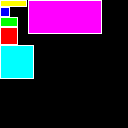
\includegraphics[width=5cm]{results02}
\end{minipage}

\subsubsection{Problemi 3 e 4}
\begin{minipage}{\textwidth}
\centering
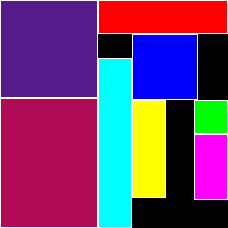
\includegraphics[width=5cm]{results03}
\hspace{1cm}

\includegraphics[width=5cm]{results04}
\end{minipage}

\subsubsection{Problemi 5 e 6}
\begin{minipage}{\textwidth}
\centering

\includegraphics[width=5cm]{results05}
\hspace{1cm}
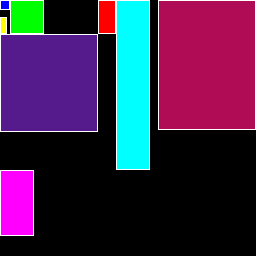
\includegraphics[width=5cm]{results06}
\end{minipage}






\iffalse

114 MIP simplex iterations
0 branch-and-bound nodes
D = 128

128
'a',93,0,16,16,0
'b',85,0,8,16,0
'c',77,0,8,8,0
'd',72,0,5,25,0
'e',0,0,72,32,0
'f',0,32,32,32,0



110 MIP simplex iterations
0 branch-and-bound nodes
D = 128

128
'a',0,27,18,18,0
'b',0,17,18,10,1
'c',0,7,10,10,0
'd',0,0,27,7,1
'e',28,0,74,34,0
'f',0,45,34,34,0






16295 MIP simplex iterations
2405 branch-and-bound nodes
D = 228

228
'a',98,0,130,34,0
'b',194,100,34,34,0
'c',132,34,66,66,0
'd',132,100,34,98,1
'e',194,134,34,66,0
'f',98,58,34,170,1
'g',0,98,98,130,0
'h',0,0,98,98,0



1084 MIP simplex iterations
277 branch-and-bound nodes
D = 224

224
'a',32,0,128,32,0
'b',192,0,32,32,0
'c',96,64,64,64,0
'd',0,192,96,32,0
'e',0,0,32,64,0
'f',56,32,168,32,0
'g',0,64,96,128,0
'h',97,128,96,96,0






4403 MIP simplex iterations
1423 branch-and-bound nodes
D = 198

198
'a',180,0,18,34,0
'b',164,164,34,34,0
'c',170,0,10,10,0
'd',169,83,7,17,0
'e',136,0,34,66,0
'f',0,0,34,170,1
'g',34,100,130,98,1
'h',34,0,98,98,0



222 MIP simplex iterations
0 branch-and-bound nodes
D = 256

256
'a',98,0,18,34,0
'b',10,0,34,34,0
'c',0,0,10,10,0
'd',0,17,7,17,0
'e',0,170,34,66,0
'f',116,0,34,170,1
'g',158,0,98,130,0
'h',0,34,98,98,0


\fi






	\newpage

